\documentclass[tikz,border=3mm]{standalone}
\usepackage{amsmath,amssymb}
\renewcommand{\familydefault}{\sfdefault}
\usepackage{tikz}
\usepackage{pgfplots}
\pgfplotsset{compat=1.18}
\usetikzlibrary{
  arrows.meta,
  positioning,
  calc,
  fit,
  backgrounds,
  shapes.geometric,
  pgfplots.fillbetween
}

\definecolor{R7Navy}{HTML}{17324D}
\definecolor{R7Teal}{HTML}{0A8F8F}
\definecolor{R7Gold}{HTML}{E0A12B}
\definecolor{R7Coral}{HTML}{D85D55}
\definecolor{R7Violet}{HTML}{6757C7}
\definecolor{R7Sky}{HTML}{5AA6C8}
\definecolor{R7Ink}{HTML}{243746}
\definecolor{R7Muted}{HTML}{667784}
\definecolor{R7Pale}{HTML}{EEF4F5}
\definecolor{R7Warm}{HTML}{FFF6E5}
\definecolor{R7Paper}{HTML}{FCFDFD}

\tikzset{
  r7box/.style={
    rounded corners=2.2mm,
    very thick,
    align=center,
    minimum height=23mm,
    text width=29mm,
    inner sep=3.2mm
  },
  r7arrow/.style={
    -{Stealth[length=2.4mm,width=1.8mm]},
    line width=1.0pt,
    color=R7Muted
  },
  r7tag/.style={
    font=\bfseries\scriptsize,
    text=R7Navy,
    fill=white,
    inner sep=1.2pt
  }
}

\pgfplotsset{
  r7axis/.style={
    axis line style={R7Ink, line width=0.8pt},
    tick style={R7Ink, line width=0.7pt},
    tick label style={font=\footnotesize, text=R7Ink},
    label style={font=\small, text=R7Ink},
    title style={font=\bfseries\small, text=R7Navy, yshift=1mm},
    grid=both,
    major grid style={draw=R7Muted!22, line width=0.45pt},
    minor grid style={draw=R7Muted!10, line width=0.35pt},
    legend style={
      draw=none,
      fill=white,
      fill opacity=0.92,
      text opacity=1,
      font=\scriptsize,
      cells={anchor=west}
    }
  }
}

\begin{document}
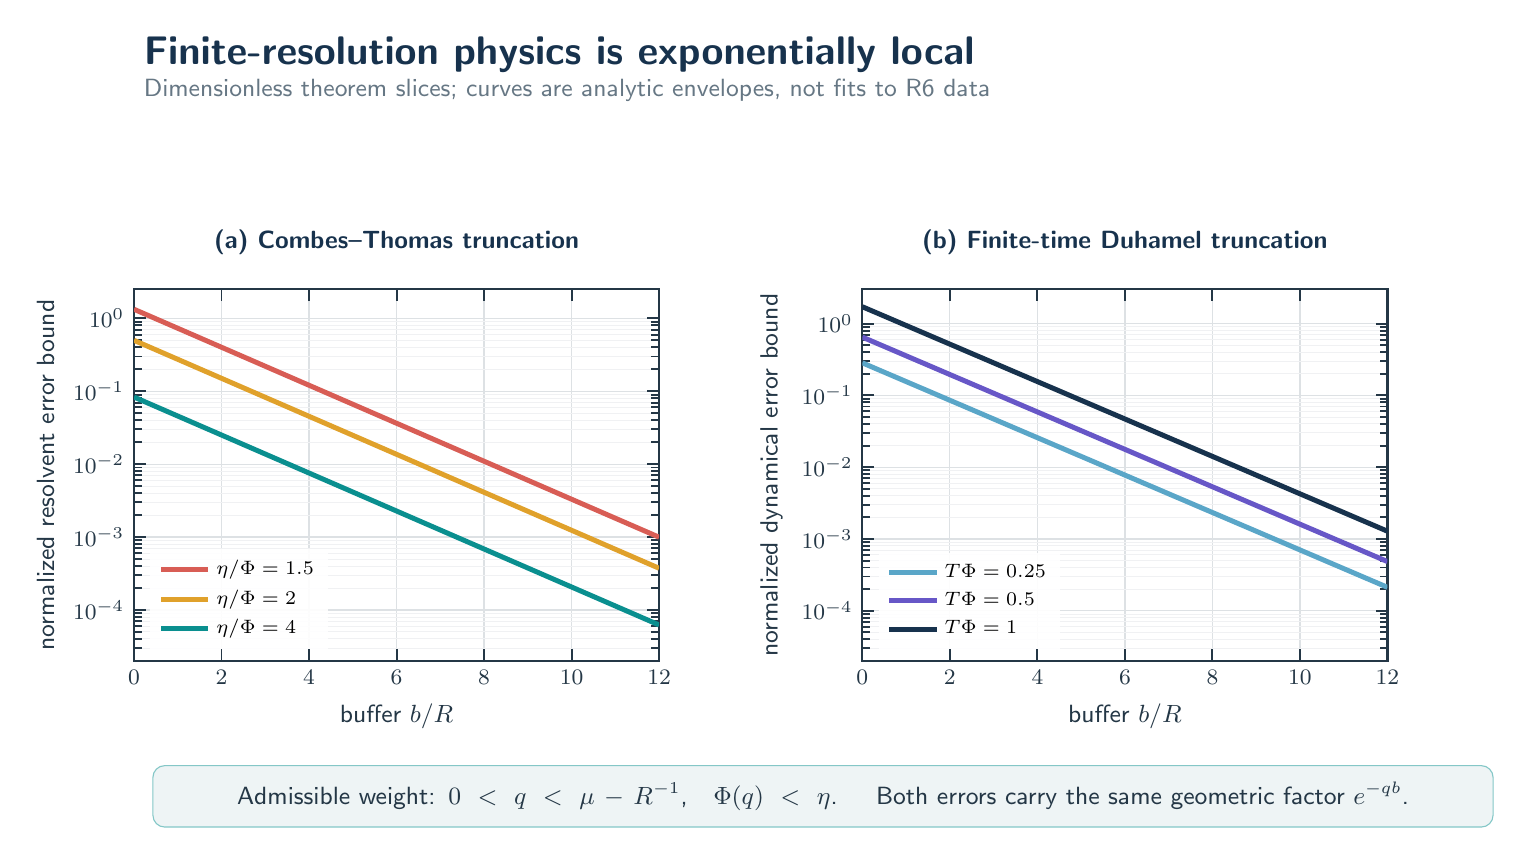
\begin{tikzpicture}[font=\sffamily]
  \node[anchor=west,font=\bfseries\Large,text=R7Navy] at (0,7.7)
    {Finite-resolution physics is exponentially local};
  \node[anchor=west,font=\small,text=R7Muted] at (0,7.25)
    {Dimensionless theorem slices; curves are analytic envelopes, not fits to R6 data};

  \begin{axis}[
    r7axis,
    at={(0,0)},
    anchor=south west,
    width=8.25cm,
    height=6.3cm,
    ymode=log,
    xmin=0,xmax=12,
    ymin=2e-5,ymax=2.5,
    xlabel={buffer $b/R$},
    ylabel={normalized resolvent error bound},
    title={(a) Combes--Thomas truncation},
    legend pos=south west
  ]
    \addplot[domain=0:12,samples=180,line width=1.8pt,R7Coral]
      {exp(-0.6*x)/(1.5*(1.5-1))};
    \addlegendentry{$\eta/\Phi=1.5$}
    \addplot[domain=0:12,samples=180,line width=1.8pt,R7Gold]
      {exp(-0.6*x)/(2*(2-1))};
    \addlegendentry{$\eta/\Phi=2$}
    \addplot[domain=0:12,samples=180,line width=1.8pt,R7Teal]
      {exp(-0.6*x)/(4*(4-1))};
    \addlegendentry{$\eta/\Phi=4$}
  \end{axis}

  \begin{axis}[
    r7axis,
    at={(9.25cm,0)},
    anchor=south west,
    width=8.25cm,
    height=6.3cm,
    ymode=log,
    xmin=0,xmax=12,
    ymin=2e-5,ymax=3,
    xlabel={buffer $b/R$},
    ylabel={normalized dynamical error bound},
    title={(b) Finite-time Duhamel truncation},
    legend pos=south west
  ]
    \addplot[domain=0:12,samples=180,line width=1.8pt,R7Sky]
      {exp(-0.6*x)*(exp(0.25)-1)};
    \addlegendentry{$T\Phi=0.25$}
    \addplot[domain=0:12,samples=180,line width=1.8pt,R7Violet]
      {exp(-0.6*x)*(exp(0.5)-1)};
    \addlegendentry{$T\Phi=0.5$}
    \addplot[domain=0:12,samples=180,line width=1.8pt,R7Navy]
      {exp(-0.6*x)*(exp(1)-1)};
    \addlegendentry{$T\Phi=1$}
  \end{axis}

  \node[rounded corners=1.5mm,draw=R7Teal!50,fill=R7Pale,
    text width=16.6cm,align=center,inner sep=2.1mm,font=\small,text=R7Ink]
    at (8.75,-1.72) {
      Admissible weight:
      $0<q<\mu-R^{-1}$,\quad $\Phi(q)<\eta$.
      \quad Both errors carry the same geometric factor $e^{-qb}$.
    };
\end{tikzpicture}
\end{document}
